\section{\textsc{Cucumber salad}}

\subsection*{Zutaten für 2 Portionen:}

\begin{tabular}{p{7.5cm} p{7.5cm}}
	& \\
	\sfrac{1}{2} cucumber & 2tbsp olive oil \\
	1tbsp vinegar & 1tbsp sugar \\
	\multicolumn{2}{l}{salt, papper, dill to taste}
\end{tabular}

\subsection*{Serving suggestion:}

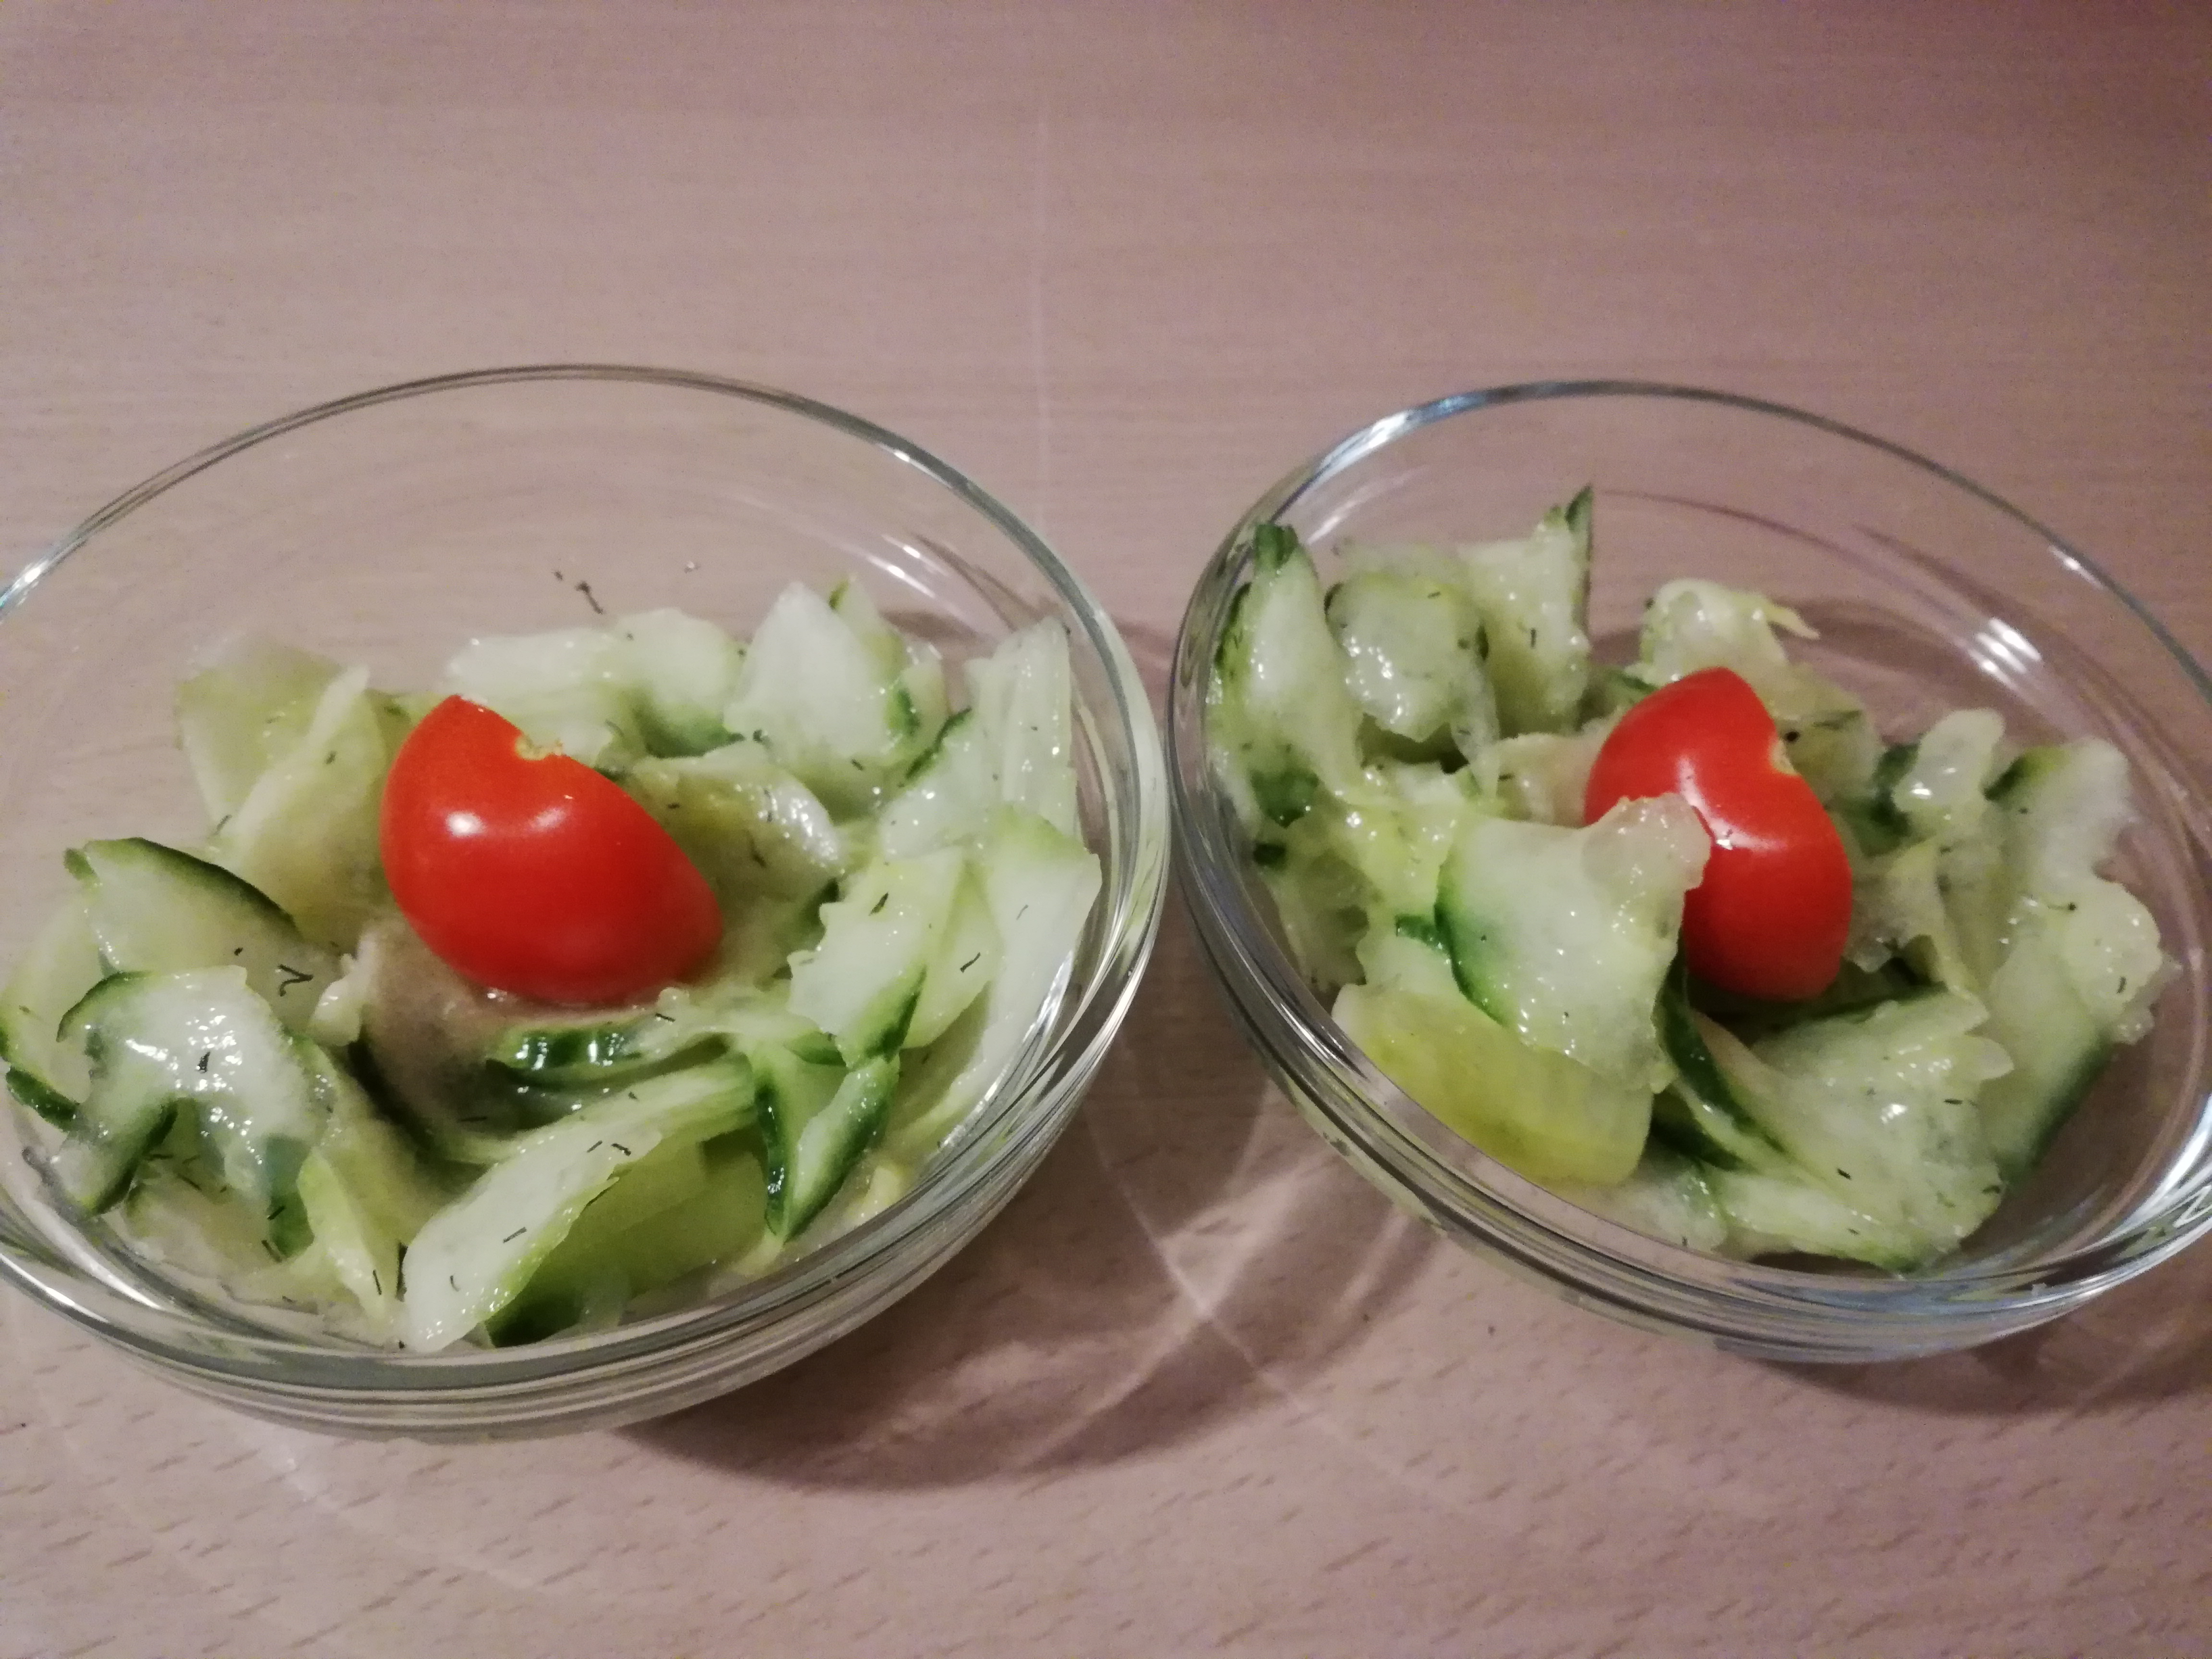
\includegraphics[width=\textwidth]{img/gurkensalat/gurkensalat_fertig.jpg} \cite{gurkensalat}

\subsection*{How it's done:}

\begin{tabular}{p{15cm}}
	\\
  Partially peel half of the cucumber with a peeler.\\
  This creates a dash of colour in the finished salad.\\
  Add the spices and oils and leave to stand for about 2 hours.
\end{tabular}
